\chapter{\label{chap:intro}Análise e Discussão}
 




\section{Resultados da \textit{Survey}}

Após a conclusão do processo de coleta dados, com o objetivo de entender quais são as preocupações de desenvolvedores de software móveis no desenvolvimento de aplicações, destaca-se nessa seção o resultado obtido na survey. A survey teve um total de 20 respondentes, o que pode indicar um possível viés nos resultados das amostras, devido ao baixo número de respondentes.

O público que respondeu essa pesquisa tem em média 5 anos de experiência com desenvolvimento de aplicações  para dispositivos móveis. Os desenvolvedores em sua maioria tinham experiência com a plataforma Android:Java, entretanto vale ressaltar as demais plataformas também (Figura \ref{fig:plataformas}). A contribuição dos desenvolvedores ocorre em sua maioria no desenvolvimento de aplicativos de uso empresarial, junto com outros tipos menores de contribuição (Figura \ref{fig:contribuicao}), com o desenvolvimento realizado em equipe 85{\%} das vezes (Figura \ref{fig:equipe}).
%falar das oturas pçataformas e dos aplicativos desenvolvidos

\begin{figure}[!b]
\vspace{1.8cm}
\centering
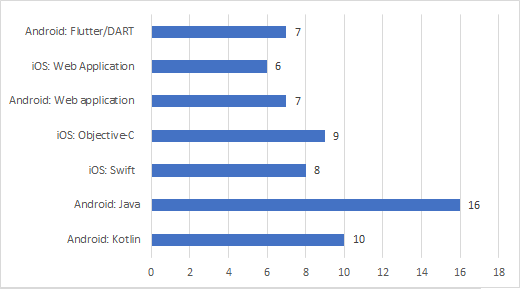
\includegraphics[scale=0.8]{fig/plataformas.PNG}
\caption{Respostas dos desenvolvedores - Plataformas mais utilizadas}
\label{fig:plataformas}

\end{figure}

\begin{figure}[H]
\centering
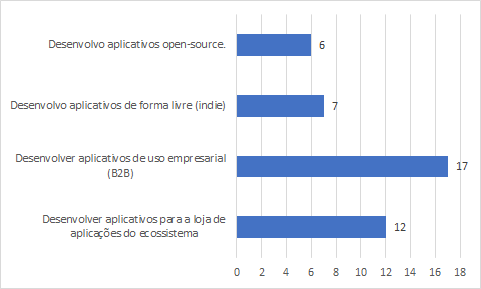
\includegraphics[scale=0.8]{fig/contribuicao.PNG}
\caption{Respostas dos desenvolvedores - Tipo de contribuição realizada}
\label{fig:contribuicao}
\end{figure}

\begin{figure}[H]
\vspace{1.8cm}
\centering
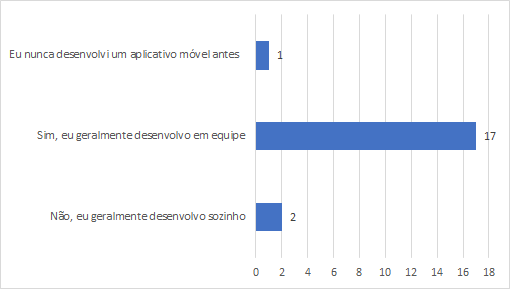
\includegraphics[scale=0.8]{fig/devjunto.png}
\caption{Respostas dos desenvolvedores - Desenvolvimento em equipe}
\label{fig:equipe}
\end{figure}

Os resultados apresentados neste capítulo expressam as respostas dos desenvolvedores sobre o questionários. Os resultados podem ser consultados na Figura \ref{fig:1} (Controle de Acesso), \ref{fig:2} (Criptografia), \ref{fig:3} (segurança das operações) e \ref{fig:4} (Aquisição, desenvolvimento e manutenção de sistemas). Os números nas células correspondem a quantidade de desenvolvedores que concordaram, discordaram ou não souberam responder.

A organização dos resultados está na mesma ordem dos controles da ISO 27002, a fim de facilitar a leitura, mantendo um sequência lógica. A seguir serão discutidos os resultados de como os desenvolvedores avaliam as questões dos controles da ISO 27002. 

\begin{figure}[H]
\centering
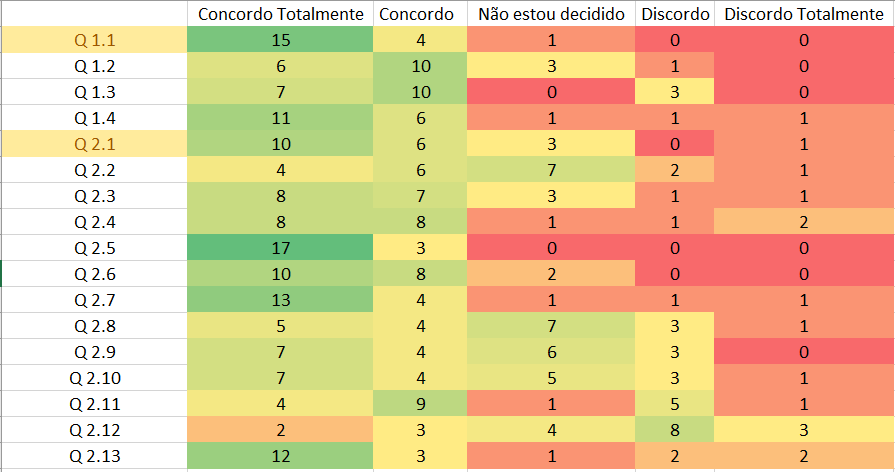
\includegraphics[scale=0.8]{fig/Mapa de calor 1.PNG}
\caption{Respostas dos desenvolvedores - Controle de Acesso}
\label{fig:1}
\end{figure}

\paragraph{ A seção 9 da norma ISO 27002, discorre sobre boas práticas de criptografia e tem como objetivo limitar o acesso à informação e aos recursos de processamento da informação, assegurar acesso de usuário autorizado e prevenir acesso não autorizado a sistemas, serviços e aplicações.  Percebe-se pelas respostas desta \textit{survey} que as questões Q1.1, Q1.2, Q1.3, Q1.4, Q2.1, Q2.3, Q2.4, Q2.5, Q2.6, Q2.7 e Q2.13 são importantes para os desenvolvedores mobile. Por outro lado, as questões Q2.8 e Q2.11, não foram consideradas relevantes pelos desenvolvedores, a questão Q2.2 foi inconclusiva no seu resultado e as questões 2.9, Q2.10 e Q2.12 tiveram um resultado positivo quanto a preocupação, porém pouco expressivo, indicando que os desenvolvedores colocam a responsabilidade da segurança ao acesso nas mãos dos próprios usuários ou não se preocupam com ela.}

\noindent\textbf{Política de controle de acesso:}

\paragraph{\textbf{(Q 1.1)} - Preocupo-me com o controle de acesso de usuários nos sistemas que desenvolvo.}


Noventa e cinco por cento (95{\%}) dos respondentes concordam que o controle de acesso em sistemas desenvolvidos é importante, considerando tanto aqueles que concordam totalmente (85{\%}) quanto aqueles que consideram a questão importante (10{\%}). Com esse resultado fica claro que existe uma preocupação dos desenvolvedores mobile com o controle de acesso de usuários.


\paragraph{\textbf{(Q 1.2)} - Preocupo-me em criar ou utilizar funcionalidades que permitam o bloqueio, remoção ou desabilitação rápida de usuários no sistema (por exemplo, funcionários que deixaram a empresa).}

Oitenta por cento (80{\%}) dos respondentes concordam que criar funcionalidades que permitam remoção, bloqueio, ou desabilitação de usuários é importante, considerando tanto aqueles que concordam totalmente (30{\%}) quanto aqueles que consideram a questão apenas importante (50{\%}). Com o resultado fica claro que existe uma preocupação dos desenvolvedores com a criação destas funcionalidades.

\vspace{0.5cm}
\noindent\textbf{Provisionamento para acesso de usuário:}

\paragraph{\textbf{(Q 1.3)} - Preocupo-me em desenvolver funções que permitam a alteração de permissão no sistema para todos os usuários, ou seja, que seja possível o gerenciamento de usuários.}


Oitenta e cinco por cento (85{\%}) dos participantes afirmam se preocupar em desenvolver funcionalidades para a alteração de permissão de usuários no sistema, considerando tanto aqueles que concordam totalmente (35{\%}), quanto aqueles que consideram a questão apenas importante (50{\%}). Com esse resultado fica claro a preocupação dos desenvolvedores com a criação de tais funcionalidades.

\paragraph{\textbf{(Q 1.4)} - Preocupo-me em criar um registro central de direitos de acesso para cada usuário, ou seja, todos os usuários possuem um ID único.}


Oitenta e cinco por cento (85{\%}) dos participantes se preocupam em criar um registro central de direitos de acesso para cada usuário, considerando tanto aqueles que concordam totalmente (55{\%}), quando aqueles que consideram apenas importante (30{\%}). Com esse resultado é possível afirmar que existe uma preocupação dos desenvolvedores com um registro central de direitos de acesso dos usuários.

\vspace{0.5cm}
\noindent\textbf{Gerenciamento da informação de autenticação secreta de usuários:}

\paragraph{\textbf{(Q 2.1)} - Preocupo-me em desenvolver funções que verifiquem a identidade de um usuário antes de fornecer uma informação de autenticação secreta, temporária, de substituição ou nova no sistema. (por exemplo e-mail de confirmação, SMS, aplicativos como Google autenticador).}

Oitenta por cento (80{\%}) dos participantes se preocupam em desenvolver funcionalidades que verifiquem a identidade de um usuário antes de fornecer informação de autenticação secreta, considerando tanto aqueles que concordam totalmente (50{\%}) , quanto aqueles que apenas concordam (30{\%}) com a questão. Com esse resultado é possível afirmar que os desenvolvedores se preocupam com a criação de funcionalidades que verifiquem a identidade do usuário.

\paragraph{\textbf{(Q 2.2)} - Preocupo-me em aprimorar o desenvolvimento de funcionalidades com autenticação secreta para acessos e logins. (autenticação por 2 fatores).}

Cinquenta por cento (50{\%}) dos participantes se preocupam em aprimorar funcionalidades de autenticação secreta em acessos nos sistemas que desenvolvem, entretanto 35{\%} não foi capaz de emitir uma opinião a respeito da pergunta e 15{\%} discorda de ser uma preocupação necessária. Com esse resultado não é capaz de afirmar se existe uma preocupação dos desenvolvedores pois grande parte do grupo não foi capaz de emitir uma opinião a respeito do tema.

\paragraph{\textbf{(Q 2.3)} - Preocupo-me para que a Informação de autenticação secreta temporária seja única para uma pessoa e que não possa ser facilmente adivinhada.}

Setenta e cinco por cento (75{\%}) dos participantes se preocupam em manter a informação de autenticação secreta única e temporária para cada pessoa, considerando tanto aqueles que concordam totalmente (40{\%}), quanto aqueles que apenas concordam (35{\%}). Com o resultado fica claro que existe uma preocupação dos desenvolvedores com o cuidado da autenticação secreta.

\vspace{0.5cm}
\noindent\textbf{Uso da informação de autenticação secreta:}
\paragraph{\textbf{(Q 2.4)} - Preocupo-me em fornecer recursos para que o usuário consiga resguardar sua privacidade durante o processo de autenticação.}

Oitenta por cento (80{\%}) dos participantes se preocupam em fornecer recursos que possibilitem ao usuário resguardar sua privacidade durante o processo de autenticação, considerando tanto aqueles que concordam totalmente (40{\%}), quanto aqueles que apenas concordam (40{\%}). Com o resultado fica claro que existe uma preocupação dos desenvolvedores em fornecer recursos que resguardem a privacidade do usuário.

\vspace{5cm}
\noindent\textbf{Procedimentos seguros de entrada no sistema (logon):}

\paragraph{\textbf{(Q 2.5)} - Preocupo-me em não mostrar dados sensíveis do usuário (status, informações pessoais, etc.) de aplicações até que o processo de Log-on tenha sido concluído com sucesso.}

Cem por cento (100{\%}) dos participantes se preocupam em não mostrar dados sensíveis dos usuários durante o processo de Log-on. Com o resultado é possível ver a unanimidade na importância que os desenvolvedores dão a essa questão.

\paragraph{\textbf{(Q 2.6)} - Preocupo-me em validar informações de entrada no sistema somente quando todos os dados de entrada estiverem completos.}

Noventa por cento (90{\%}) dos participantes se preocupam em validar os dados de entrada no sistema somente quando estiverem completos, considerando tanto aqueles que concordam totalmente (50{\%}), quanto aqueles que apenas concordam (40{\%}). Com esse resultado fica claro que existe uma preocupação dos desenvolvedores em validar os dados do usuário somente quando estiverem totalmente completos.

\paragraph{\textbf{(Q 2.7)} - Caso ocorra um erro na validação das informações de entrada me preocupo em não identificar qual parte do dado de entrada está correto ou incorreto (Ex: “Sua senha está incorreta”).}

Oitenta e cinco por cento (85{\%}) dos participantes se preocupam em não revelar qual parte do dado esta correto ou incorreto em um processo de entrada no sistema, considerando tanto aqueles que concordam totalmente (65{\%}), quanto aqueles que apenas concordam (20{\%}). Com esse resultado fica claro a preocupação do desenvolvedores em não fornecer ajuda a um usuário possivelmente mal intencionado.

\paragraph{\textbf{(Q 2.8)} - Preocupo-me em proteger o sistema contra tentativas consecutivas/repetidas de entrada forçada.}

Quarenta e cinco por cento (45{\%}) dos participantes se preocupam em proteger o sistema contra tentativas consecutiva de entrada forçada no sistema, contudo 35{\%} dos respondentes não foi capaz de opinar sobre a questão e 20{\%} discorda que seja um preocupação.Com esse resultado não é possível afirmar se existe uma preocupação dos desenvolvedores com proteção do sistema contra um tentativa forçada de entrada no sistema.

\paragraph{\textbf{(Q 2.9)} - Preocupo-me em comunicar um evento de segurança caso uma tentativa potencial ou uma violação bem sucedida de entrada no sistema (log-on), seja detectada.}

Cinquenta e cinco por cento (55{\%}) dos participantes se preocupam em comunicar eventos de segurança, contudo 30{\%} não souberam responder e 15{\%} discordaram. Com esse resultado é possível afirmar que existe uma preocupação dos desenvolvedores sobra a comunicação de eventos de segurança.

\paragraph{\textbf{(Q 2.10)} - Preocupo-me em encerrar sessões inativas após um período de inatividade.}

Cinquenta e cinco por cento (55{\%}) dos participantes se preocupam em encerrar sessões inativas após um período de inatividade, contudo 25{\%} não soube opinar e 20{\%} discordaram que seria uma preocupação. Com esse resultado é possível  ver que existe uma preocupação dos desenvolvedores quanto ao tempo de inatividade.

\vspace{0.5cm}
\noindent\textbf{Sistema de gerenciamento de senha:}
\paragraph{\textbf{(Q 2.11)} - Preocupo-me em fazer sistemas que obriguem uma escolha de senha de qualidade, por exemplo, com no mínimo Oito Caracteres, misturar letras em caixa alta e baixa com números e caracteres não alfanuméricos).}

Sessenta e cinco por cento (65{\%}) dos participantes se preocupa em obrigar o usuário a criar um senha de qualidade, entretanto 30{\%} descorda que  isso seja uma preocupação. Com o resultado é possível afirmar que existe uma preocupação dos desenvolvedores em obrigar o usuário criar senhas de qualidade, entretanto seria relevante entender o motivo que levou os 30{\%} dos participantes a discordarem da importância. 

\paragraph{\textbf{(Q 2.12)} - Preocupo-me em desenvolver sistemas que obriguem usuário a mudarem as suas senhas temporárias no primeiro acesso ao sistema (Sistema que coloca sua senha inicial como data de aniversário ou dígitos do RG).}

Cinquenta e cinto por cento (55{\%}) dos respondentes dos participantes não se preocupam em obrigar o usuário a trocar a senha temporária de primeiro acesso, 20{\%} não soube responder e Apenas 25{\%} dos participantes concordaram que obrigar a troca de senha seria uma preocupação. Com esse resultado é possível concluir que não existe uma preocupação forte dos desenvolvedores sobre essa questão.

\paragraph{\textbf{(Q 2.13)} - Preocupo-me em não permitir que a senhas possam ser mostradas na tela quando digitadas (Ex: Usar recurso do “olho” para revelar senha em um campo).}

Setenta e cinco por cento (75{\%}) dos respondentes se preocupam em resguardar a visualização da senha quando digitada.  Com esse resultado é possível  ver que existe uma preocupação dos desenvolvedores quanto a proteção da visualização da senha.





\begin{figure}[H]
\centering
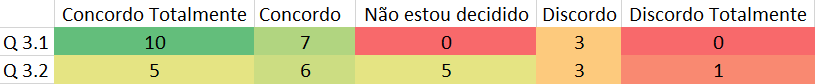
\includegraphics[scale=0.7]{fig/Mapa de calor 2.PNG}
\caption{Respostas dos desenvolvedores - Criptografia}
\label{fig:2}
\end{figure}

\paragraph{A norma ISO 27002 na sua seção 10 aborda boas práticas de criptografia que tem como objetivo assegurar o uso efetivo e adequado da criptografia para proteger a confidencialidade, autenticidade e a integridade da informação.  Das 2 questões apresentadas apenas a Q3.1 foi considerada como extremamente relevante pela grande maioria dos desenvolvedores. A questão Q3.2 foi considerada relevante, porém o resultado foi pouco expressivo, possivelmente pela complexidade sobre o tema.}

\noindent\textbf{Política para o uso de controles criptográficos:}
\paragraph{\textbf{(Q 3.1)} - Preocupo-me com uso de criptografia para a proteção das informações sensíveis durante a comunicação em dispositivos móveis.}

Oitenta e cinco por cento (85{\%}) dos participantes se preocupam usar criptografia para a proteção de informações, considerando tanto aqueles que concordam totalmente (50{\%}), quanto aqueles que apenas concordam (35{\%}). Com o resultado fica claro que existe uma preocupação dos desenvolvedores com a utilização de criptografia.

\vspace{0.5cm}

\noindent\textbf{Gerenciamento de chaves:}
\paragraph{\textbf{(Q 3.2)} - Preocupo-me em gerar chaves para diferentes sistemas criptográficos e diferentes aplicações.}

Cinquenta e cinco por cento (55{\%}) dos participantes se preocupam em gerar chaves para diferentes sistemas criptográfico, 25{\%} não souberam opinar e 20{\%} discordam que seja uma preocupação. Com esse resultado é possível ver que a maioria dos desenvolvedores considera que gerar diferentes chaves criptográficas é importante.
 
\begin{figure}[H]
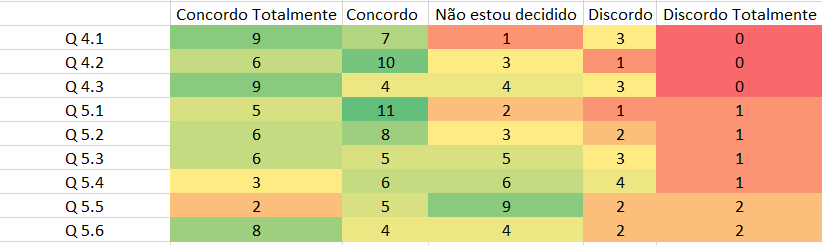
\includegraphics[scale=0.7]{fig/Mapa de calor 3.PNG}
\caption{Respostas dos desenvolvedores - Segurança das Operações }
\label{fig:3}
\paragraph{As boas práticas para garantir a segurança das operações, são apresentadas na seção 12 da Norma ISO 27002 e tem como objetivo garantir a operação segura e correta dos recursos de processamento da informação, assegurar que as informações e os recursos de processamento da informação estão protegidos contra \textit{malware}, a proteção contra perda de dados, registrar eventos e gerar evidências, assegurar a integridade dos sistemas operacionais e prevenir a exploração de vulnerabilidades técnicas e minimizar o impacto das atividades de auditoria nos sistemas operacionais. Percebe-se pelas respostas que as questões Q4.1, Q4.2, Q4.3, Q5.1, Q5.2 e Q5.6 foram as mais importantes para os desenvolvedores mobile, o que demonstra uma preocupação relevante quanto a operação segura e correta dos recursos de processamento e registro de eventos. Por outro lado, as questões  Q5.4 e Q5.5 não foram consideradas como uma preocupação, o que indica uma preocupação desnecessária e a questão Q5.3 foi considerada relevante, porém o resultado foi pouco expressivo, o que indica uma possível falta de preocupação sobre as questões.}
\end{figure}

\noindent\textbf{Responsabilidades e procedimentos operacionais:}
\paragraph{\textbf{(Q 4.1)} - Preocupo-me com os impactos na segurança da informação quando ocorre alguma mudança no sistema.}

Oitenta por cento (85{\%}) do participantes se preocupam com os impactos da segurança da informação quando ocorre alguma mudança no sistema, considerando tanto aqueles que concordam totalmente (45{\%}), quanto aqueles que apenas concordam (35{\%}).Com esse resultado fica claro que existe uma preocupação dos desenvolvedores.

\vspace{4cm}
\noindent\textbf{Gestão de capacidade:}
\paragraph{\textbf{(Q 4.2)} - Preocupo-me em criar mecanismos para atender o crescimento da aplicação e possibilitar suportar demanda variável de acessos.}

Oitenta por cento (80{\%}) dos participantes se preocupam em criar mecanismos para atender o crescimento da aplicação, considerando tanto aqueles que concordam totalmente (30{\%}), quanto aqueles que apenas concordam (50{\%}).Com esse resultado fica claro que existe uma preocupação dos desenvolvedores.

\vspace{0.5cm}
\noindent\textbf{Separação dos ambientes de desenvolvimento, teste e de produção:}
\paragraph{\textbf{(Q 4.3)} - Preocupo-me para que dados sensíveis não sejam copiados para os ambientes de testes.}

Sessenta e cinco por cento (65{\%}) dos participantes se preocupam em não copiar dados sensíveis para o ambiante de teste, considerando tanto aqueles que concordam totalmente (45{\%}), quanto aqueles que apenas concordam (20{\%}).Com esse resultado fica claro que existe uma preocupação dos desenvolvedores em não copiar dados sensíveis para o ambiente de teste. 

\vspace{0.5cm} 
\noindent\textbf{Registros de eventos:}
\paragraph{\textbf{(Q 5.1)} - Preocupo-me em criar mecanismos para registrar os eventos do sistema.}

Oitenta por cento (85{\%}) dos participantes se preocupam em criar mecanismos para registrar eventos no sistema, considerando tanto aqueles que concordam totalmente (45{\%}), quanto aqueles que apenas concordam (20{\%}). Com esse resultado fica claro que existe uma preocupação dos desenvolvedores em registrar os eventos no sistema.

\paragraph{\textbf{(Q 5.2)} -Preocupo-me com datas, horários e detalhes de eventos-chave, como, por exemplo, horário de entrada (log-on) e saída (log-off) no sistema.}

Setenta por cento (70{\%}) dos participantes se preocupam em registrar eventos de entrada e saída do sistema, considerando tanto aqueles que concordam totalmente (30{\%}), quanto aqueles que apenas concordam (40{\%}).Com esse resultado fica claro que existe uma preocupação dos desenvolvedores em registrar os eventos de datas e horários.

\paragraph{\textbf{(Q 5.3)} -Preocupo-me com a identificação do dispositivo ou sua localização quando possível e o identificador do sistema.}

Cinquenta e cinco por cento (55{\%}) dos participantes se preocupam com localização ou identificação dos dispositivos, 25{\%} não soube opinar e 20{\%} discaram que seja uma preocupação. Com o resultado é possível ver que a maioria dos desenvolvedores se preocupa com a questão, entretanto uma parcela significativa não soube responder ou discordou.

\paragraph{\textbf{(Q 5.4)} - Preocupo-me com registro de tentativas de acesso ao sistema, aceitas e rejeitadas.}

Quarenta e cinco por cento (45{\%}) dos participantes se preocupam em registrar tentativas de acesso ao sistema, 30{\%} não soube opinar e 25{\%} não acha que seja uma preocupação. Com o resultado não fica possível afirmar se existe uma preocupação dos desenvolvedores a respeito da questão.


\paragraph{\textbf{(Q 5.5)} - Preocupo-me com a coleta dos endereços e protocolos de rede no log.}

Trinta e cinco por cento (35{\%}) dos participantes se preocupam com a coleta de endereços e protocolos de rede, 45{\%} não soube opinar e 20{\%} não consideram como uma preocupação. Com o resultado não é possível afirmar se existe uma preocupação dos desenvolvedores, pois a maior parte dos respondentes não soube responder a questão.

\vspace{0.5cm}
\noindent\textbf{Proteção das informações dos registros de eventos (logs):}
\paragraph{\textbf{(Q 5.6)} - Preocupo-me para que arquivos de log não sejam editados ou excluídos sem a devida autorização.}

Sessenta por cento (60{\%}) dos participantes se preocupam com integridade dos arquivos de log,considerando tanto aqueles que concordam totalmente (40{\%}), quanto aqueles que apenas concordam (20{\%}). Com esse resultado é possível observar que existe uma preocupação dos desenvolvedores com a integridade dos logs.


\begin{figure}[H]
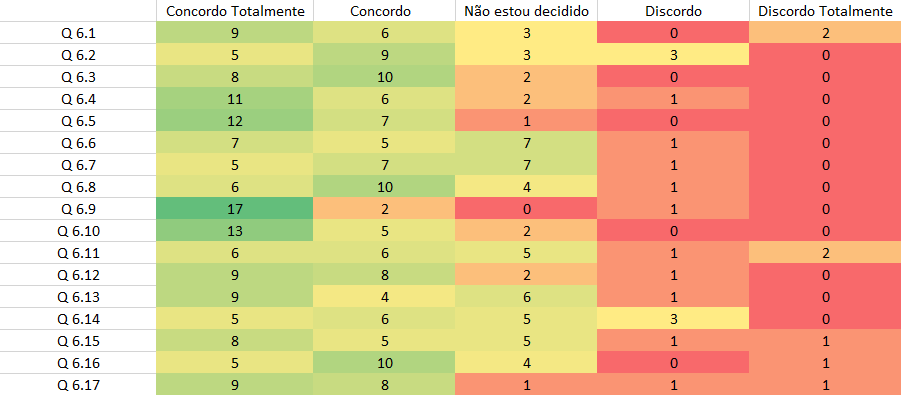
\includegraphics[scale=0.7]{fig/Mapa de calor 4.PNG}
\caption{Respostas dos desenvolvedores - Aquisição, Desenvolvimento e Manutenção de Sistemas}
\label{fig:4}
\paragraph{A seção 14 da ISO 27002 apresenta as boas práticas para  garantir a aquisição, desenvolvimento e manutenção de sistemas com o objetivo de garantir que a segurança da informação seja parte integrante de todo o ciclo de vida dos sistemas de informação, garantir que a segurança da informação esteja projetada e implementada no ciclo de vida de desenvolvimento dos sistemas de informação e assegure a proteção dos dados usados para teste. Percebe-se pelas respostas desta \textit{survey}, que as questões Q6.1, Q6.2, Q6.3 Q6.4, Q6.5, Q6.8, Q6.9, Q6.10, Q6.11, Q6.12, Q6.13, Q6.15,Q 6.16, Q6.17 são consideradas como preocupações pelos desenvolvedores, o que pode significar que os mesmo já adotam tais práticas durante o desenvolvimento. Entretanto questões como a Q6.6, Q6.7 e Q6.14 não tiveram uma unanimidade sobre a preocupação nas respostas. É importante ressaltar que os números de respostas neutras em relação as demais opções foi consideravelmente alto nas questões Q6.6 e Q6.7, o que pode indicar falta de entendimento sobre o assunto ou a necessidade de elaborar melhor a questão.}
\end{figure}

\noindent\textbf{Análise e especificação dos requisitos de segurança da informação:}
\paragraph{\textbf{(Q 6.1)} - Preocupo-me em identificar falhas de segurança nas aplicações móveis que dou manutenção.}

Setenta e cinco por cento (75{\%}) dos participantes se preocupam em identificar falhas de segurança, considerando tanto aqueles que concordam totalmente (40{\%}), quanto aqueles que apenas concordam (20{\%}). Com esse resultado é possível observar que existe uma preocupação dos desenvolvedores.


\vspace{0.5cm}
\noindent\textbf{Serviços de aplicação seguros sobre redes públicas:}
\paragraph{\textbf{(Q 6.2)} - Preocupo-me para que as informações envolvidas nos serviços de aplicação que transitam em redes que são de acesso público sejam protegidas de atividades fraudulentas, disputas contratuais e divulgações e modificações não autorizadas.}

Setenta por cento (70{\%}) dos participantes se preocupam com as informações envolvidas nos serviços de aplicação em redes publicas, considerando tanto aqueles que concordam totalmente (25{\%}), quanto aqueles que apenas concordam (45{\%}). Com esse resultado é possível afirmar que a maior parte dos desenvolvedores se preocupam em proteger informações em redes públicas.

\vspace{0.5cm}
\noindent\textbf{Protegendo as transações nos aplicativos de serviços:}
\paragraph{\textbf{(Q 6.3)} - Preocupo-me em usar protocolos de comunicação seguros para obter uma transação segura e confidencial.}

Noventa por cento (90{\%}) dos participantes se preocupam em usar protocolos de comunicação seguros para manter a confidencialidade. Com esse resultado fica claro que existe uma preocupação dos desenvolvedores mobile com a utilização de protocolos seguros.

\paragraph{\textbf{(Q 6.4)} - Preocupo-me em evitar que os detalhes da transação fiquem em um meio de armazenamento acessível diretamente pela internet, sem a devida segurança.}

Oitenta e cinco por cento (85{\%}) dos participantes se preocupam em evitar que os detalhes de uma transação fiquem em uma armazenamento acessível diretamente pela internet. Com esse resultado fica claro que existe uma preocupação dos desenvolvedores mobile com o armazenamento de transações seguras.

\paragraph{\textbf{(Q 6.5)} - Preocupo-me em utilizar repositórios seguros para construção de aplicações.}

Noventa e cinco por cento (95{\%}) dos participantes se preocupam utilizar repositórios seguros. Com esse resultado fica claro que existe uma preocupação dos desenvolvedores mobile.

\vspace{3cm}
\noindent\textbf{Política de desenvolvimento seguro:}
\paragraph{\textbf{(Q 6.6)} - Preocupo-me com a análise dos controles da aplicação e dos procedimentos de integridade para assegurar que eles não tenham sido comprometidos pelas mudanças na plataforma operacional.}

Sessenta por cento (60{\%}) dos participantes se preocupam, com a análise dos controles da aplicação, contudo {35\%} não soube responder.Com esse resultado é possível mostrar que existe uma preocupação dos desenvolvedores mobile, entretanto o número considerável de respostas neutras pode indicar que a questão não estivesse claro ou falta de entendimento.


\vspace{0.5cm}
\noindent\textbf{Análise crítica técnica das aplicações após mudanças nas plataformas operacionais:}
\paragraph{\textbf{(Q 6.7)} - Preocupo-me em analisar novas tecnologias para serem aplicadas para reduzir os riscos de segurança.}

Sessenta por cento (60{\%}) dos participantes se preocupam em analisar novas tecnologias para redução de riscos de segurança e {35\%} não soube opinar. Com esse resultado é possível afirmar que a maioria dos desenvolvedores se preocupa, entretanto o número considerável de respostas neutras pode indicar que a questão não estivesse claro ou falta de entendimento.


\vspace{0.5cm}
\noindent\textbf{Princípios para projetar sistemas seguros:}
\paragraph{\textbf{(Q 6.8)} - Preocupo-me em analisar os riscos (impacto/probabilidade) para prover o desenvolvimento de segurança na aplicação.}

Oitenta por cento (80{\%}) do participantes se preocupam em analisar riscos de impacto para prover o desenvolvimento de segurança na aplicação, considerando tanto aqueles que concordam totalmente (30{\%}), quanto aqueles que apenas concordam (50{\%}). Com esse resultado fica claro que existe uma preocupação dos desenvolvedores mobile.

\paragraph{\textbf{(Q 6.9)} - Preocupo-me em separar diferentes ambientes de desenvolvimento (dev/ teste /prod ).}

Noventa e cinco por cento (95{\%}) dos respondentes se preocupam em separar os ambientes de desenvolvimento,considerando tanto aqueles que concordam totalmente (85{\%}), quanto aqueles que apenas concordam (10{\%}).Com esse resultado fica evidente a preocupação dos desenvolvedores mobile com a separação dos ambientes. Com esse resultado fica claro que existe uma preocupação dos desenvolvedores mobile.


\vspace{0.5cm}
\noindent\textbf{Ambiente seguro para desenvolvimento:}
\paragraph{\textbf{(Q 6.10)} - Preocupo-me com a sensibilidade dos dados a serem processados, armazenados e transmitidos pelo sistema.}

Noventa por cento (90{\%}) dos participantes se preocupam com a sensibilidade dos dados, considerando tanto aqueles que concordam totalmente (65{\%}), quanto aqueles que apenas concordam (25{\%}). Com esse resultado fica claro que existe uma preocupação dos desenvolvedores mobile.

\paragraph{\textbf{(Q 6.11)} - Preocupo-me em realizar testes de segurança em funcionalidades desenvolvidas.}

Sessenta por cento (60{\%}) dos participantes se preocupam em realizar testes de segurança em funcionalidades desenvolvidas, 25{\%} não soube responder e 15{\%} discordam que seja uma preocupação. Com esse resultado é possível ver que existe uma preocupação dos desenvolvedores em realizar testes de segurança.


\vspace{0.5cm}
\noindent\textbf{Teste de segurança do sistema:}
\paragraph{\textbf{(Q 6.12)} - Preocupo-me em realizar testes unitários.}

Oitenta e cinco por cento (85{\%}) dos respondentes se preocupam em realizar testes unitários, considerando tanto aqueles que concordam totalmente (45{\%}), quanto aqueles que apenas concordam (40{\%}). Com esse resultado fica claro que existe uma preocupação dos desenvolvedores mobile.

\paragraph{\textbf{(Q 6.13)} - Preocupo-me em realizar testes das funcionalidades desenvolvidas, de maneira integrada no sistema.}

Sessenta e cinco por cento (65{\%}) dos respondentes se preocupam em realizar testes de maneira integrada no sistema e 30{\%} não souber opinar. Com esse resultado é possível ver que existe uma preocupação dos desenvolvedores mobile, entretanto a quantidade de pessoal que não souberam opinar pode indicar que questão pudesse ser melhor elaborada

\paragraph{\textbf{(Q 6.14)} - Preocupo-me em utilizar ferramentas de análise de código.}

Cinquenta e cinco por cento (55{\%}) dos participantes se preocupam em utilizar ferramentas de análise de código, 25{\%} não soube responder e 20{\%} discordam que seja uma preocupação. Com o resultado é possível ver que a maioria dos desenvolvedores se preocupa, entretanto uma quantidade considerável não soube opinar ou discordou.

\vspace{0.5cm}
\noindent\textbf{Teste de aceitação de sistemas:}
\paragraph{\textbf{(Q 6.15)} - Preocupo-me em realizar testes de aceitação de sistemas.}

Sessenta e cinco por cento (65{\%}) dos entrevistados se preocupam em realizar testes de aceitação, 25{\%} não soube responder e 10{\%} discordou que que fosse uma preocupação. Com o resultado é possível ver a maioria dos desenvolvedores se preocupa com a realização de testes de aceitação.

\paragraph{\textbf{(Q 6.16)} - Preocupo-me em cuidados dos dados de testes, caso o banco de dados operacional seja utilizado.}

Setenta e cinco por cento (75{\%}) dos participam se preocupam com proteção dos dados de teste, caso o banco operacional seja utilizado, ,considerando tanto aqueles que concordam totalmente (25{\%}), quanto aqueles que apenas concordam (50{\%}).  Com esse resultado é possível ver que existe uma preocupação dos desenvolvedores.

\vspace{0.5cm}
\noindent\textbf{Proteção dos dados para teste:}
\paragraph{\textbf{(Q 6.17)} - Preocupo-me em proteger os dados do banco de dados operacional contra remoção e modificação.}

Oitenta e cinco por cento (85{\%}) dos participantes se preocupam em proteger os dados do banco operacional. Com esse resultado é possível ver que existe uma preocupação dos desenvolvedores com esses aspectos.